\section{Technical appendices and supplementary material}
\label{sec:appendix}
\subsection{Stage1 Model Selection}

\begin{figure*}[h]
\centering
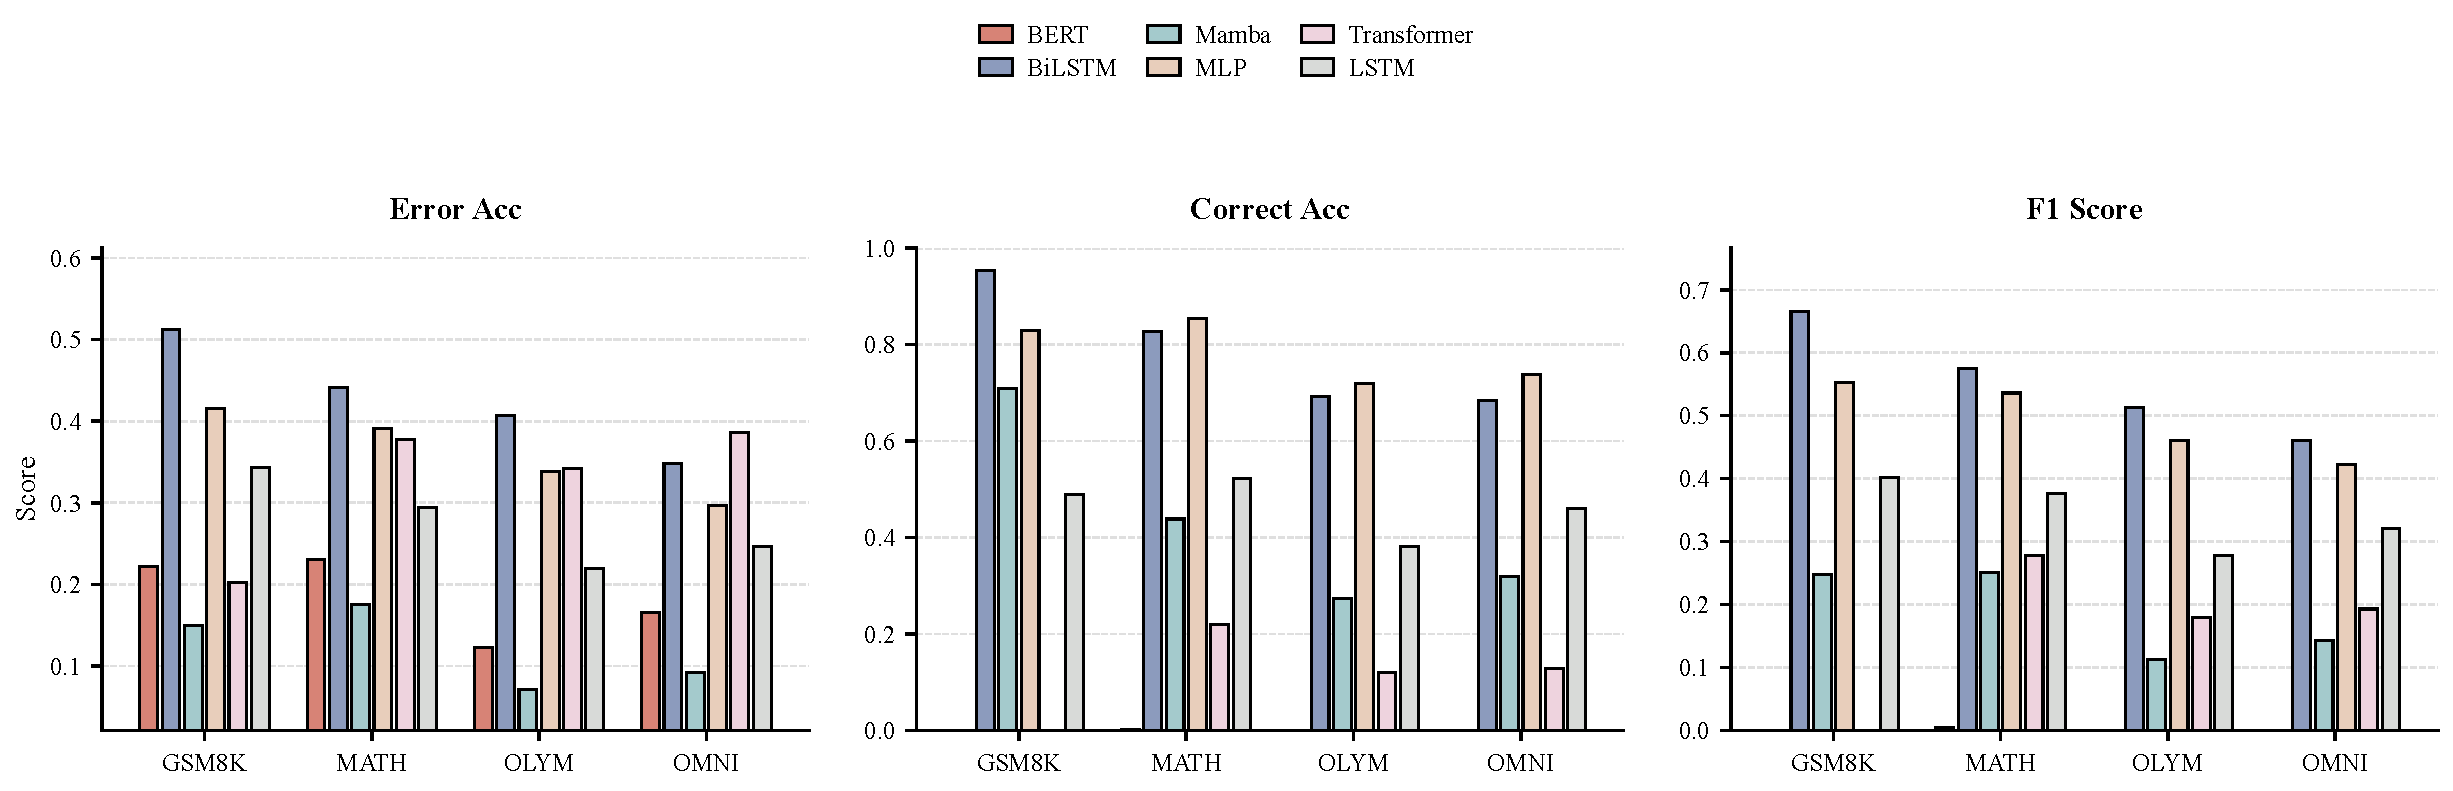
\includegraphics[width=\textwidth]{figures/model_selection_all_metrics.pdf}
\caption{Stage 1 model selection across all metrics. Different reward-scorer architectures are compared under the same feature input and optimization setup.}
\label{fig:stage1_model_selection}
\end{figure*}

As shown in Figure~\ref{fig:stage1_model_selection}, we evaluate multiple architectures as the Stage 1 Final Reward Scorer by measuring downstream PRM performance on ProcessBench. For all models except BERT, we use step-level feature representations as input. For BERT, we aggregate integrated gradients over each step's token span at the embedding level. For the Transformer scorer, we test max pooling, mean pooling, and attention-weighted fusion, and report the attention-weighted variant. For the MLP scorer, we test max and mean pooling and report mean pooling.

The results suggest that compressed step-level representations are necessary: BERT obtains nearly zero F1, indicating that direct embedding-level attribution introduces mostly noisy and ineffective gradients. BiLSTM consistently outperforms LSTM across metrics, showing that global context is beneficial for modeling cross-step dependencies. Notably, MLP performs closest to BiLSTM; we hypothesize that MLP preserves more complete information for gradient integration, whereas BiLSTM preserves more task-relevant information and vanilla LSTM forgets some useful cues.

\subsection{Input Feature Selection}
\label{step_features_selection}

\begin{figure*}[t]
    \centering
    % --- 子图 (a) ---
    \begin{subfigure}[t]{0.32\textwidth}
        \centering
        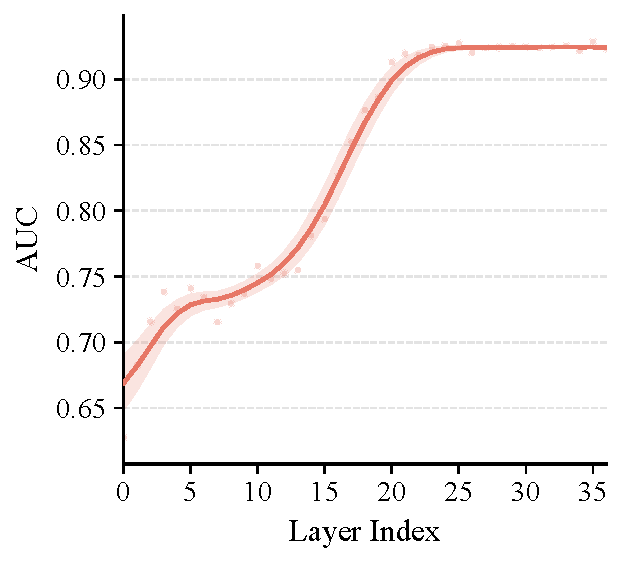
\includegraphics[width=\linewidth]{figures/mlp_layers_auc.pdf}
        \caption{Layer-wise AUC.}
        \label{fig:mlp_layers_auc}
    \end{subfigure}
    \hfill
    % --- 子图 (b) ---
    \begin{subfigure}[t]{0.32\textwidth}
        \centering
        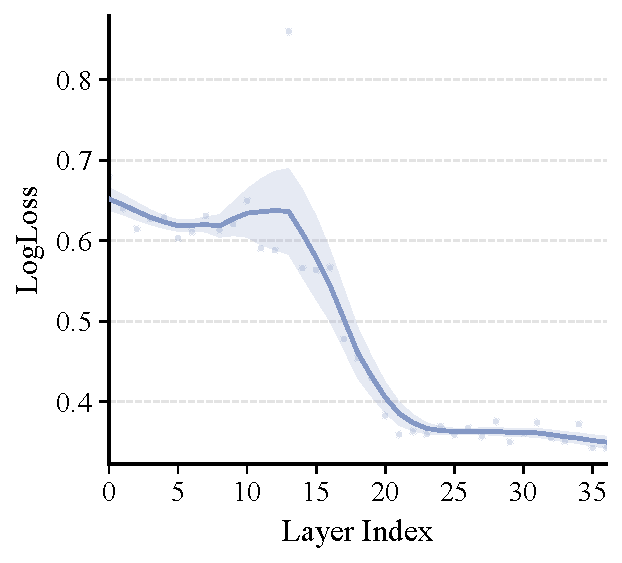
\includegraphics[width=\linewidth]{figures/mlp_layers_logloss.pdf}
        \caption{Layer-wise log-loss.} % 删掉 performance，让标题更简洁
        \label{fig:mlp_layers_loss}
    \end{subfigure}
    \hfill
    % --- 子图 (c) ---
    \begin{subfigure}[t]{0.32\textwidth}
        \centering
        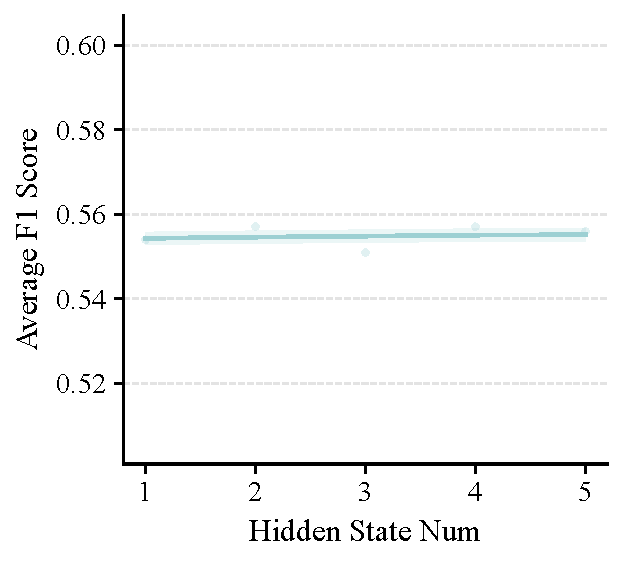
\includegraphics[width=\linewidth]{figures/multi_hidden_f1.pdf}
        \caption{F1 vs. hidden states.} % 精简长标题
        \label{fig:multi_hidden}
    \end{subfigure}

    \caption{Input feature selection layout: (a) AUC analysis, (b) log-loss analysis, and (c) F1 score variation on ProcessBench.}
    \label{fig:input_feature_selection}
\end{figure*}

In this section, we investigate three key questions regarding the step representation $x_{i, t} \in \mathbb{R}^{d}$: which single hidden layer provides the optimal representation, how many layers should be combined, and whether prefix differencing is beneficial. To determine which layers best capture step semantics, we conduct linear-probe experiments by training the Final Reward Scorer on hidden states extracted from various layers. Furthermore, we train PRMs using varying numbers of hidden layers and evaluate the impact of differential versus raw inputs through qualitative case studies.

As illustrated in Figure~\ref{fig:input_feature_selection}(a) and (b), linear-probe experiments reveal that representations from deeper layers (those closer to the output) are significantly more effective for Stage 1 trajectory-correctness prediction, with both AUC and log-loss converging to optimal levels in the final layers. Moreover, Figure~\ref{fig:input_feature_selection}(c) demonstrates that concatenating hidden states from multiple top layers yields no observable improvement in the downstream PRM F1 score. Consequently, we strictly utilize the single final-layer hidden state for step representation, maximizing computational efficiency without compromising performance.

To address the differential-input question, we analyze specific reasoning cases. Figure~\ref{fig:case_study} % TODO: 替换为Case Study
illustrates an erroneous trajectory where a critical mistake occurs at Step 1. Although subsequent steps maintain local computational consistency, they stem from a flawed premise and must ultimately be judged as incorrect. Our analysis reveals that raw hidden states better preserve global logical coherence by retaining full contextual history, whereas prefix differencing aggressively discards crucial cross-step dependencies.

\subsection{IG Baseline Selection}
\label{ig_baseline_selection}
To choose the IG baseline, we consider two options: (i) using the first-order
forward-difference feature vector $x_{i,t-1}$ as the baseline for the current
step, and (ii) using randomly initialized vectors as semantically empty
baselines.

The motivation for option (i) is to capture incremental step contribution.
In this case, for input $X_i=[x_{i,0},\ldots,x_{i,T_i}]$, the baseline sequence
is $X_{i}^{baseline}=[x_{i,-1}, x_{i,0}, \ldots, x_{i,T_i-1}]$, where
$x_{i,-1}$ denotes a manually defined baseline for the question-boundary state,
interpreted as a semantically uninformative vector.
IG completeness then gives:

\begin{equation}
\label{baseline_selection_delta}
\sum_{t=0}^{T_i}\delta_{\text{local}}^{\mathrm{IG}}(s_{i,t})
=
F(x_{i,0}:x_{i, T_i}) - F(x_{i,-1}:x_{i, T_{i-1}}),
\end{equation}

In Stage 1, the objective is to predict trajectory score from step-level features, so $F(x_{i,-1}:x_{i, T_{i-1}})$ can be interpreted as the score prediction of a right-shifted trajectory. The resulting IG signal therefore attributes steps relative to this shifted context, which is semantically misaligned with our intended notion of stepwise marginal contribution. For this reason, we do not adopt option (i).

For option (ii), summing per-step IG signals gives:
\begin{equation}
\label{baseline_selection_zero}
\sum_{t=0}^{T_{i}}\delta_{\text{local}}^{\mathrm{IG}}(s_{i,t}) 
= 
F(x_{i,0}:x_{i, T_i}) - F(x_{i,0}^{baseline}:x_{i, T_{i}}^{baseline}),
\end{equation}

According to the IG definition, each step attribution reflects its contribution relative to the baseline prediction. In \citep{sundararajan2017axiomatic}, $x^{baseline}$ is set to the all-zero vector for image attribution, with the goal of using a minimally informative state to avoid biased attributions. In process-reward modeling with binary outcome signals ($0/1$), we define a minimally informative baseline as one producing near-neutral output, i.e., $F(X^{baseline})\approx0.5$, so that attribution signs directly indicate whether a step is beneficial or harmful. Comparing an all-zero baseline with random-noise baselines, we find that the all-zero baseline yields outputs stably close to $0.5$, whereas random baselines are less stable. We therefore adopt the all-zero baseline, which preserves completeness and the semantics of feature-level integrated gradients, and best matches the Aumann--Shapley perspective.


\subsection{Global Delta Analysis}

\begin{figure*}[h]
\centering
\begin{minipage}[c]{0.48\textwidth}
    \centering
    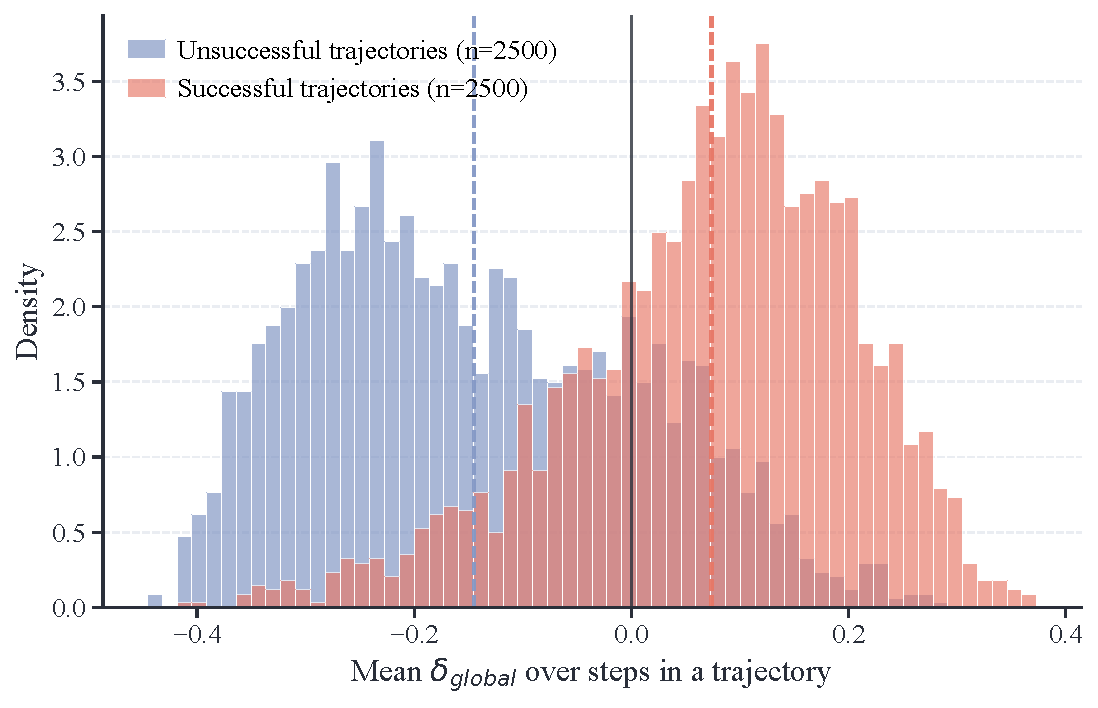
\includegraphics[width=\linewidth, height=0.6\textwidth, keepaspectratio]{figures/traj_mean_delta_by_reward.pdf}
    \\[-1mm]
    {\footnotesize\textbf{(a)} Mean global delta by reward group.}
\end{minipage}\hfill
\begin{minipage}[c]{0.48\textwidth}
    \centering
    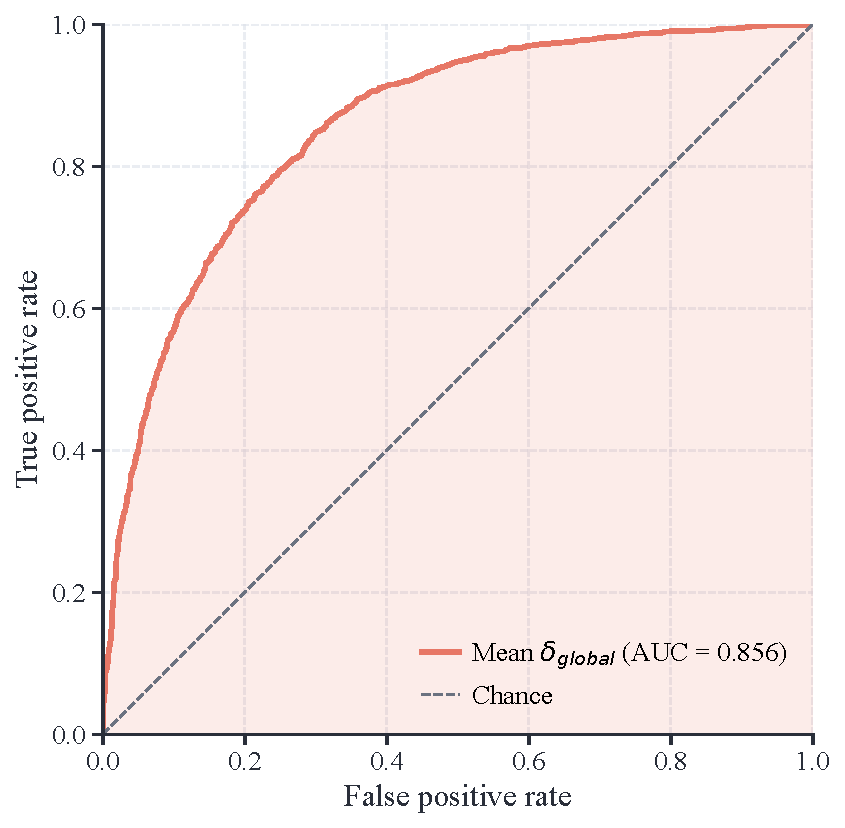
\includegraphics[width=\linewidth, height=0.6\textwidth, keepaspectratio]{figures/traj_roc_mean_delta.pdf}
    \\[-1mm]
    {\footnotesize\textbf{(b)} ROC curve using mean global delta.}
\end{minipage}
\caption{Global delta analysis with two trajectory-level views.}
\label{fig:global_delta_analysis}
\end{figure*}

To empirically validate the efficacy of the proposed global signal $\delta_{\text{global}}$, we analyze its trajectory-level distribution and predictive capacity. Recall from our formulation that $\delta_{\text{global}}(s_{i,t})$ acts as a cross-trajectory empirical prior, approximating the relative success tendency of specific semantic patterns via nearest-neighbor voting. 

Figure~\ref{fig:global_delta_analysis}(a) illustrates the distribution of the mean global signal—aggregated over all steps within an individual trajectory—stratified by the final episodic return ($n=2500$ for each group). The empirical distributions exhibit a clear and substantial separation. Successful trajectories are predominantly characterized by a positive mean $\delta_{\text{global}}$, whereas unsuccessful trajectories consistently yield negative values. This observation aligns seamlessly with our theoretical premise: state representations associated with successful outcomes reliably retrieve high-reward neighbors from the cross-trajectory candidate pool $\Omega$, confirming that $\delta_{\text{global}} > 0$ effectively encodes a higher-than-average propensity for success.

To rigorously quantify the discriminative power of this prior, Figure~\ref{fig:global_delta_analysis}(b) presents the Receiver Operating Characteristic (ROC) curve for predicting the binary final reward $r \in \{0, 1\}$ solely using the trajectory-mean $\delta_{\text{global}}$. The estimator achieves an Area Under the Curve (AUC) of 0.856, demonstrating strong predictive performance significantly above random chance. 

Collectively, these results substantiate the utility of our non-parametric voting estimator. By surfacing robust, cross-sample statistical constraints, the global signal provides a highly discriminative empirical prior that fundamentally complements the intra-trajectory marginal contributions ($\delta_{\text{local}}$) within our Shapley framework.